\section{Diag MC for the Froehlich Polaron}
In chapter 2 we have seen that is possible to perturbatively expand the Matsubara Green's function for the Froehlich polaron 
in a series of integrals \ref{GF_expansion_integral}, while in chapter 3 we have shown that series of this type can be computed 
using a special type of Markov chain Monte Carlo called Diagrammatic Monte Carlo which is able to take into account all the possible 
perturbative expansions of the full function and sample from it.\\
We now focus on the specific Diagrammatic Monte Carlo technique employed for the Froehlich Polaron case. Let us consider the 
Froehlich Hamiltonian $H^{cFr}$ in the specific case of a single anisotropic electron band and multiple phonon modes. We take into account 
the non-interacting term
\begin{equation}
    H^{cFr}_0=\sum_{\mathbf{k}}\left(\frac{k^2}{2m(\hat{k})}-\mu\right)c^\dagger_{\mathbf{k}}c_{\mathbf{k}}+\sum_{\mathbf{q}j}\omega_{jLO}a^\dagger_{\mathbf{q}j}a_{\mathbf{q}j},
\end{equation}
where we are only taking into account the electron polaron (the only difference in the hole polaron case would be negative electron energy dispersion). The chemical potential 
$\mu$ is put inside the electron term as a renormalization constant (\textbf{fictitious potential renormalization} \cite{mishchenko2000diagrammatic})\cite{fehske2007computational} which can be tuned in order to obtain a non-divergent distribution that decays 
as an exponential for long $\tau$ in the stationary limit.\\\
The interaction term reads:
\begin{equation}
    V^{cFR}=\sum_{\mathbf{k},\mathbf{q}j}c^\dagger_{\mathbf{k+q}}c_{\mathbf{k}}\left(V^{cFr}_{\mathbf{q}j}a_q+V^{*cFr}_{\mathbf{q}j}a^\dagger_{-\mathbf{q}}\right),
\end{equation}
where the interaction vertex $V^{cFr}$ has formula
\begin{equation}
    V^{cFr}_{\mathbf{q}j}=\frac{i}{q}\frac{4\pi}{\Omega_0}\left(\frac{1}{2\omega_{jLO}V_{BvK}}\right)^{1/2}\frac{p_j}{\epsilon^{\infty}}.
\end{equation}
We need a technique to translate the Green's functions defined in chapter 2 to the formalism of Diagrammatic Monte Carlo. To this aim 
we identify the stationary distribution $Q(\left\{y\right\})$ with the two Green's function of interest: the one-electron Green's function 
$G(\mathbf{k},\tau)$, where no external phonon lines are present:
\begin{equation}
\begin{split}
    G(\mathbf{k},\tau)=\sum_{n=0,2,4,...}^{+\infty}\sum_{\xi_n}\int d\tau_1\cdots \int d\tau_n\int d\mathbf{q}_1 \frac{V_{q_1j_1}}{(2\pi)^3}\cdots\int d\mathbf{q}_{n/2}\frac{V_{q_{n/2}j_{n/2}}}{(2\pi)^3} \\
    \times D_n^{\xi_n}(\mathbf{k},\tau;\tau_1,...,\tau_{n},\mathbf{q}_1,...,\mathbf{q}_{n/2},j_1,...,j_{n/2}),
\end{split}
\end{equation}
and $P(\mathbf{k},\tau)$, a function that is the sum of the single electron Green's function and all the possible one-electron $N$-phonons Green's function 
configurations (weighted accordingly):
\begin{equation}
    P(\mathbf{k},\tau)=G(\mathbf{k},\tau)+\sum_{N=1}^{+\infty}G^{(N)}(\mathbf{k}\tilde{\mathbf{q}}_1,...,\tilde{\mathbf{q}}_N, j_1,...,j_N,\tau),
\end{equation}
where $G^{(N)}(\mathbf{k},\tau)$ is diagrammatically expanded in 
\begin{equation}
\begin{split}
   &G^{(N)}(\cdots)=\sum_{\xi_n}\int d\tau_1\cdots \int d\tau_n\int d\mathbf{q}_1\frac{V_{q_1j_1}}{(2\pi)^3}\cdots\int d\mathbf{q}_{n/2}\frac{V_{q_{n/2}j_{n/2}}}{(2\pi)^3}\\
    &\times D_n^{\xi_n}(\mathbf{k},\tilde{\mathbf{q}}_1,...,\tilde{\mathbf{q}}_N,\tilde{j}_1,...,\tilde{j}_N,\tau;\tau_1,...,\tau_n,\mathbf{q}_1,...,\mathbf{q}_{n/2},j_1,...,j_{n/2}).
\end{split}
\end{equation}
It is now important to distinguish between external variables ${y}$ and the internal ones $\{x_1,...,x_n\}$. We identify them as
\begin{equation}
\begin{split}
    \{&y\}\to \{\mathbf{k},\tilde{\mathbf{q}}_1,\tilde{j}_1,...,\tilde{\mathbf{q}}_N,\tilde{j}_N, \tau \},\\
    &n\to \{0,2,4,...\},\\
    \{&x_1,...,x_n\}\to \{\tau_1,...,\tau_n, \mathbf{q}_1, j_1,..., \mathbf{q}_{n/2}, j_{n/2}\}.
\end{split}
\end{equation}
The algorithm that computes our simulation must satisfy the ergodicity requirement of Markov chain Monte Carlo: for this reason it 
is necessary to implement updates that change the external variables $\{y\}$, the internal ones $\{x_i\}$, and the order of the diagram 
$n$.\\
We start by saying that no updates have been implemented in order to sample from the free electron momentum $\mathbf{k}$, which will be fixed 
for each individual simulation: this was made in order to have a more precise control about the region of $k-space$ that we want to simulate, in particular 
the $\mathbf{k}=0$ point where the electron is at the bottom (top) of the conduction (valence) band.\\
The chemical potential $\mu$ is also implemented in the simulations as a normalizing factor, in this way a free electron propagator 
becomes:
\begin{equation}
    G_0(\mathbf{k},\tau)\to G_0(\mathbf{k}, \mu, \tau)=e^{-(\epsilon(\mathbf{k})-\mu)\tau},
\end{equation}
the effect of which can be easily reversed by rescaling the result.\\
Due to the finite memory of computers, it is then necessary to fix for each simulation a maximum imaginary time value $\tau_{max}$, a maximum 
internal order $n_{max}$ (the number of internal phonon propagators would be $n_{max}/2$) and a maximum number of external phonon propagators $N_{max}$.\\
Having decided this, it is then necessary to state the electron effective mass on the three main axes $m^*_{x}$, $m^*_{y}$ and $m^*_{z}$ together with 
the number of phonon modes that couple to the electron band $n_{ph}$ together with their energy $\omega_{jLO}$ and their phonon mode polarities 
$p_j$ or another equivalent quantity from which their value can be recovered \cite{de2023high}.\\
Other quantities that needs to be specified are the size of the unit cell $\Omega_0$, the size of the Born-von Karman cell $V_{BvK}$, the optical 
dielectric tensor (a scalar in the case of cubic materials) $\epsilon_{\infty}$, the number of thermalization steps $N_{relax}$ set to achieve the 
stationary distribution condition and the number of simulation steps $N_{steps}$.\\
It is now important to define how the diagram was effectively modelled in the computer: to this aim three data structures were 
defined.
The \textbf{Vertex}: this data structure encapsulates all the data which describes the vertices of the electron-phonon interaction (also the diagram beginning and end)
together with all the relevant information about the associated phonon propagator, its components are:
\begin{itemize}
    \item $\tau_i$, the imaginary time value of the vertex, 0 and $\tau$ for the extrema
    \item \textbf{type}, integer parameter which differentiates between extrema (0), internal phonon vertices (+1 for outgoing phonon propagators 
    and -1 for incoming ones), external phonon vertices (+2 for outgoing phonon propagators and -2 for incoming ones).
    \item \textbf{linked}, integer value which shows to which other vertex the current vertex is linked to and thus the length of the 
    phonon propagator (whether we have an internal or external one).
    \item $\mathbf{q}_i$, the three momentum components of the free phonon propagator which is created or annihilated at the vertex.
    \item \textbf{index}, the phonon mode which is involved in the electron-phonon interaction at the vertex. 
\end{itemize}
The \textbf{Propagator}: this data structure represents the free electron propagators, it is defined by the three electron momentum components 
$\mathbf{k}_i$.\\
The \textbf{Effective\_Mass}: this data structure represents the effective mass $m^*_i(\hat{k})$ of the electron for each electron propagator $\mathbf{k}_i$, 
it is computed using the formula in \ref{effective_mass_anisotropic_relation}.\\
At the start of each simulation, an array of dimension $n_{max}+2N_{max}+2$ of Vertex data type is created, while an array of dimension 
$n_{max}+2N_{max}+1$ is created for the Propagator and Effective\_Mass data type. At the beginning of the simulation all the single elements of the three data types 
are initialized to default values with the exception of the first 2 Vertex elements and the first Propagator and Effective\_Mass 
element: the latter two are initialized using the $\mathbf{k}$ value given as input and by computing the related effective mass (default to 
1 in the case that $\mathbf{k}=0$), while the $\tau$ values of the first two Vertex elements are initialized to 0 and $\tau$ respectively, where 
$\tau$ is retrieved using the \textbf{Diagram Length} update, which will be explained in detail in the following section.
\subsection{Updates}
Updates are necessary to obtain a Markov chain for the system which is ergodic, there is no single way to implement them in order to 
achieve this aim and different choices have been proposed about the way new parameters are proposed and how updates are implemented 
\cite{mishchenko2000diagrammatic}\cite{hahn2018diagrammatic}, here it is thus shown just a proposal that is sufficient but is nevertheless not 
necessarily the best or fastest choice.\\
The first update that is described is the \textbf{Diagram Length} update (class I), which updates the length of the last electron propagator: it thus changes the +
value of the external variable $\tau$.\\
Since the last electron propagator is a free electron propagator, which decays exponentially with $\tau$ as
\begin{equation}
    G_0(\mathbf{k},\tilde{\mathbf{q}}_1,...,\tilde{\mathbf{q}}_N,\tau)=\exp{ \left\{-\left(\frac{p^2}{2m^*(\hat{p})}-\sum_{j}\omega_{jLO}n_{jph}-\mu \right)(\tau-\tau_{last})\right\}},
    \label{free_propagator_electron_final}
\end{equation}
with $\tau_{last}$ time of last vertex before the diagram end, and where we have:
\begin{equation}
\begin{split}
    \mathbf{p}=\mathbf{k}-\sum_{i=0}^N\tilde{\mathbf{q}}_i,\\
    \sum_j n_{jph}=N,
\end{split}
\end{equation}
with $N$ total number of external phonons in the current diagram and $j$ phonon mode index.\\
The weight ratio between two diagrams with length $\tau$ and $\tau'$ thus becomes:
\begin{equation}
    \frac{D_n(\cdots,\tau')}{D_n(\cdots,\tau)}=\frac{e^{-\Delta E (\tau'-\tau_{last})}}{e^{-\Delta E (\tau-\tau{last})}},
    \label{weights_diagram_length}
\end{equation}
where $\Delta E$ is the computed energy in \ref{free_propagator_electron_final}.
\begin{figure}[H]
    \centering
    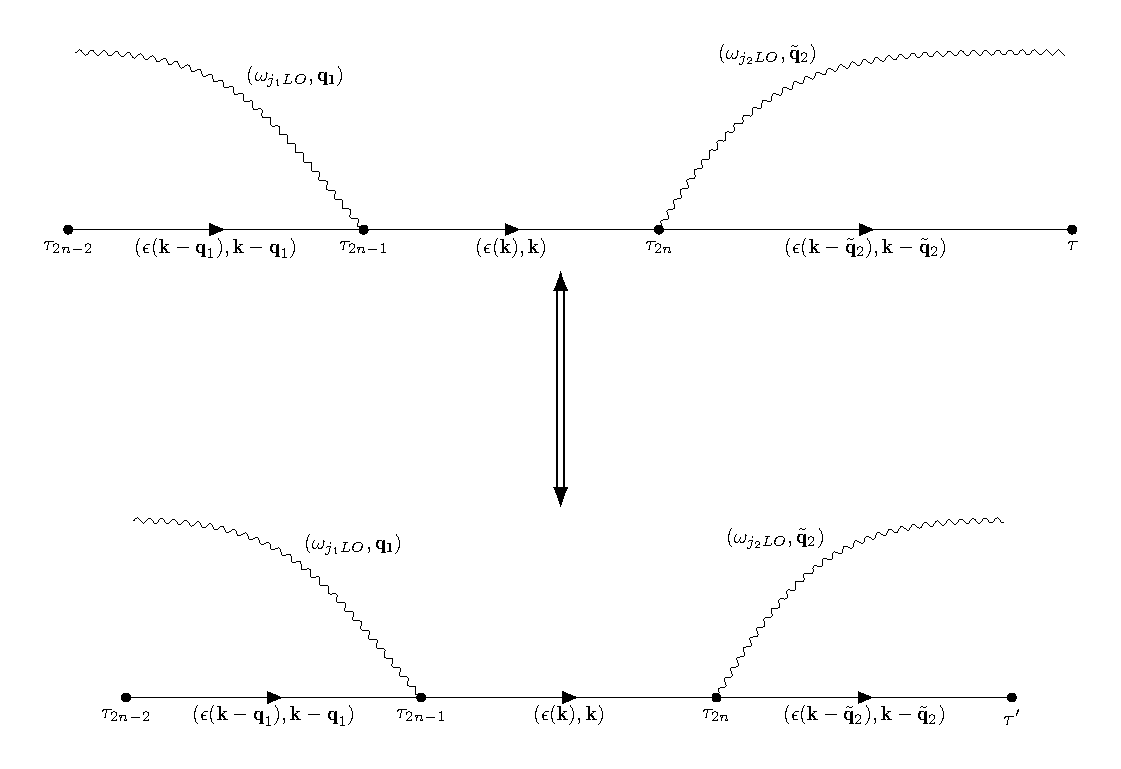
\includegraphics[scale=0.6]{diagram_length_v2.pdf}
    \caption{Diagram length update.}
    \label{fig:length_update}
\end{figure}
If we thus take an exponential distribution as the proposal distribution for new values of the imaginary time value $\tau'$ built as follows
\begin{equation}
    \tau'=\tau_{last}-\frac{\log{\left(1-r\right)}}{\Delta E},
\end{equation}
with $r$ uniform random variable in $[0,1]$ we obtain a new value that is always accepted apart from the case where $\tau'>\tau_{max}$. In fact the acceptance ratio is
\begin{equation}
    R_{\tau'\tau}=\frac{\exp{\left(\tau;\tau_{last},\Delta E\right)}e^{-\Delta E(\tau'-\tau_{last})}}{\exp{\left(\tau';\tau_{last},\Delta E\right)}e^{-\Delta E (\tau-\tau_{last})}}=\frac{\Delta E e^{-\Delta E(\tau-\tau_{last})}e^{-\Delta E (\tau'-\tau_{last})}}{\Delta E e^{-\Delta E(\tau'-\tau_{last})}e^{-\Delta E (\tau-\tau_{last})}}=1,
\end{equation}
which is always accepted.\\
The next update to be described is the \textbf{add internal phonon}, a class II update. The new (internal) variables that have to be proposed 
are the time value of the outgoing vertex $\tau'$, the time value of the incoming vertex $\tau''$, the phonon mode index $j$ and the phonon propagator 
momentum $\mathbf{q}$. If proposing the diagram means that $n+2>n_{max}$ maximum allowed internal order, then the update is rejected.\\
An electron propagator (from the first one to the last for a total of $n+1$ possible choices) is chosen at random, then the value of $\tau'$ is generated 
using a uniform distribution between $\tau_{left}$ and $\tau_{right}$ vertices of the chosen free electron propagator.\\
The phonon mode $j$ is then chosen at random between the ones given in input, and the value of the second vertex of the phonon propagator $\tau''$ is generated using the
following exponential distribution
\begin{equation}
    P(\tau''|\tau',j)=\tau'-\frac{\log(1-r)}{\omega_{jLO}},
\end{equation}
where $\tau''$ is not restrained to any particular free electron propagator. The update is straight-up rejected if $\tau''>\tau$ length of the 
full diagram or if it is too close to another vertex ($|\tau''-\tau_i|<10^{-9}$).\\
The phonon momentum values $\mathbf{q}$ are then proposed using a probability $P(\mathbf{q}|\tau',\tau'',j)$ dependent on a gaussian distribution with 
mean $0$ and variance $(\tau''-\tau')^{-1}$.\\
The ratio of the two diagrams are
\begin{equation}
\begin{split}
    &\frac{D_{(n+2)}(\mathbf{k},\tau,...,\tau',\tau'',\mathbf{q},...)}{D_{n}(\mathbf{k},\tau,...)}=\\
    =&\exp{\left\{-\left(\sum_i\epsilon(\mathbf{k}_i-\mathbf{q})-\epsilon(\mathbf{k}_i)\Delta\tau_i-\omega_{LO}(\tau''-\tau')\right)\right\}}|V_{\mathbf{q}j}|^2d\tau'd\tau''\frac{d\mathbf{q}}{(2\pi)^3},
\end{split}
\end{equation}
where the sum over $i$ is extended over all the phonon propagators between the two phonon vertices $\tau'$ and $\tau''$, while $\Delta\tau_i$ is computed as $\tau_i-\tau_{i-1}$ where the two 
extrema are $\tau'$ and $\tau''$. The infinitesimal are required because they are not cancelled in the ratio since they are new proposed variables.\\
The full distribution from which the new values are sampled is written as
\begin{equation}
\begin{split}
    &P(\tau',\tau'',\mathbf{q},j)=P(\tau')P(\tau''|\tau',j)P(\mathbf{q}|\tau',\tau'',j)=\\
    &=\underbracket[1.5pt][3pt]{\frac{1}{\tau_{right}-\tau_{left}}}_{P(\tau')}\underbracket[1.5pt][3pt]{\omega_{jLO}e^{-\omega_{jLO}(\tau''-\tau')}}_{P(\tau''|\tau',j)}
    \underbracket[1.5pt][3pt]{\left(\frac{\tau''-\tau'}{2\pi}\right)^{3/2}e^{-\frac{q^2}{2}(\tau''-\tau')}}_{P(\mathbf{q}|\tau',\tau'',j)}.
\end{split}
\end{equation}
The acceptance ratio thus becomes:
\begin{equation}
    R_{add}=\frac{p_A}{p_B}\frac{D_{n+2}(\mathbf{k},\tau,...,\tau',\tau'',\mathbf{q},...)}{D_n(\mathbf{k},\tau,...)P(\tau',\tau'',\mathbf{q},j)},
\end{equation}
the context factors $p_A$ and $p_B$ take into account the number of free electron propagators from which a vertex can be generated and the total number of internal phonon propagators 
which can be removed, their ratio is
\begin{equation}
    \frac{p_A}{p_B}=\frac{p_{(rem\hspace{2pt}int)}}{p_{(add\hspace{2pt}int)}}\frac{n+2N+1}{n/2+1},
\end{equation}
for example at order $n=2$ and 1 external phonon we can choose from $2+2\cdot1+1=5$ electron propagators, while to go back to 
order 2 from order $n+2=4$ we can choose between $2/2+1=2$ phonon propagators. The two variables $p_{(rem\hspace{2pt}int)}$ and 
$p_{(add\hspace{2pt}int)}$ measure the probability of choosing the add internal and remove internal updates in the main Monte Carlo simulation.
\begin{figure}[H]
    \centering
    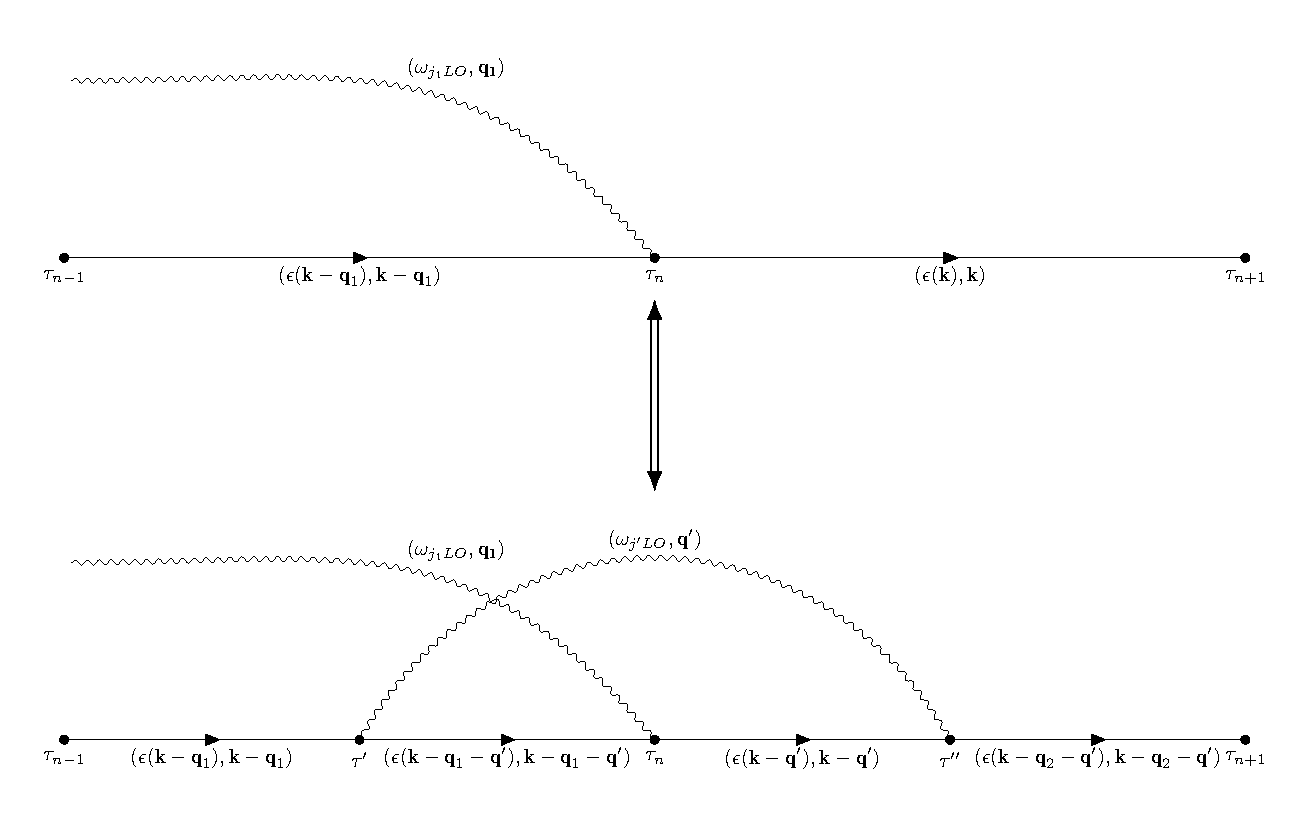
\includegraphics[scale=0.6]{add_update.pdf}
    \label{fig:add_update}
    \caption{Diagram add/remove internal phonon update.}
\end{figure}
The \textbf{remove internal phonon} is also a class II update, no new parameters are proposed but instead a random internal phonon propagator with 
vertices at $\tau'$ and $\tau''$ and momentum $\mathbf{q}$ is chosen to be removed. The update is automatically rejected if the internal order $n=0$ and 
is accepted with acceptance ratio $R_{rem}=1/R_{add}$ calculated for the add internal phonon update.
\begin{figure}[H]
    \centering
    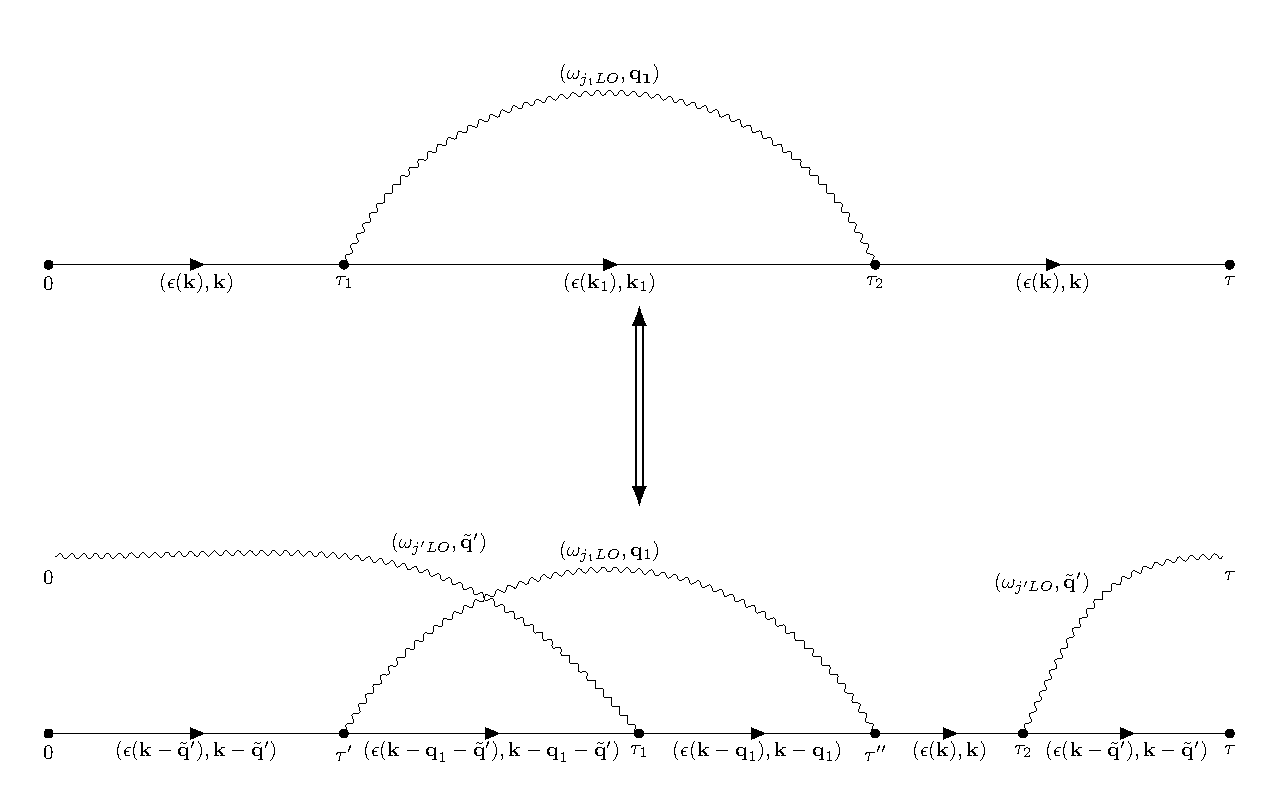
\includegraphics[scale=0.6]{add_ext_update.pdf}
    \caption{Diagram add/remove external phonon update.}
    \label{fig:diagram_add_ext}
\end{figure}
Another necessary update to implement is the \textbf{add external phonon} update, a class II update which adds an external phonon to 
the current diagram, if the number of external phonon propagators is already $N_{max}$ the update is automatically rejected.\\ 
The new variables that need to be proposed are the time values of the vertices $\tau'$ and $\tau''$, the phonon mode index 
$j$ and the phonon momentum $\tilde{\mathbf{q}}$. After having chosen the proposed phonon mode index $j$ we want to write the full probability as:
\begin{equation}
    P(\tau',\tau'',\tilde{\mathbf{q}},j)=P(\tau'|j)P(\tau''|j)P(\tilde{\mathbf{q}}|\tau',\tau'',j),
\end{equation}
in order to do so we choose the following proposal distribution for $\tau'$:
\begin{equation}
    \tau'=0-\frac{\log{\left(1-r\right)}}{\omega_{jLO}},
\end{equation}
where $r$ is a uniform random variable in $[0,1]$, if a value of $\tau'>\tau$ length of the current diagram is chosen the update is rejected. For 
$\tau''$ the following similar exponential distribution is used
\begin{equation}
    \tau''=\tau+\frac{\log{\left(1-r\right)}}{\omega_{jLO}},
\end{equation}
if $\tau''<0$ the update is directly rejected. The update is also rejected if any of the two values $\tau'$ and $\tau''$ lie too close 
to any other vertex $|\tau',\tau''-\tau_i|<10^{-9}$. New values for the momentum $\tilde{\mathbf{q}}$ are then proposed using the normal distribution 
with mean $0$ and variance $1/(\tau -\tau''+\tau')$, which takes into account the imaginary time length of the external phonon propagator.\\
The full probability thus becomes:
\begin{equation}
\begin{split}
    &P(\tau',\tau'',\tilde{\mathbf{q}},j)=P(\tau'|j)P(\tau''|j)P(\tilde{\mathbf{q}}|\tau',\tau'',j)=\\
    &=\underbracket[1.5pt][3pt]{\omega_{jLO}e^{-\omega_{jLO}\tau'}}_{P(\tau'|j)}\underbracket[1.5pt][3pt]{\omega_{jLO}e^{-\omega_{jLO}\tau''}}_{P(\tau''|j)}
    \underbracket[1.5pt][3pt]{\left(\frac{\tau-\tau''+\tau'}{2\pi}\right)^{D/2}e^{-\frac{\tilde{\mathbf{q}}}{2}(\tau-\tau''-\tau')}}_{P(\tilde{\mathbf{q}|\tau',\tau'',j})}.
\end{split}
\end{equation}
It is now important to evaluate the ratio of the two diagrams, two different cases are possible:
\begin{itemize}
    \item $\tau'<\tau''$, in this case the internal part of the two diagrams is the same
    \item $\tau'>\tau''$, here the two diagrams are completely different, in particular the free electron propagator all have different momenta.
\end{itemize}
Let us start with the first case, we have
\begin{equation}
\begin{split}
    &\frac{D_{n+2}(\mathbf{k},\tau,...,\tau',\tau'',\tilde{\mathbf{q}},...)}{D_n(\mathbf{k},\tau,...)}=\\
    =&\exp\left\{-\left(\sum_{i_1}\left[\epsilon(\mathbf{k}_{i_1}-\tilde{\mathbf{q}})-\epsilon(\mathbf{k}_{i_1})\right]\Delta\tau_{i_1}+\sum_{i_2}\left[\epsilon(\mathbf{k}_{i_2}-\tilde{\mathbf{q}})-\epsilon(\mathbf{k}_{i_2})\right]\Delta\tau_{i_2}\right)\right\}\\
    &\cdot\exp{\left\{\left(-\omega_{jLO}(\tau-\tau''+\tau')\right)\right\}}|V_{\tilde{q}j}|^2d\tau'd\tau''\frac{d\tilde{\mathbf{q}}}{(2\pi)^3},
\end{split}
\end{equation}
where $i_1$ indexes a sum over the propagators below $\tau'$, $i_2$ one over the propagators above $\tau''$, and $\Delta\tau_{i_1}$, $\Delta\tau_{i_2}$ 
are computed in the same way as performed for the add internal phonon update (considering the boundaries for the two sums as $\tau'$ and $\tau''$ respectively).\\
In the second case, we instead have the expression
\begin{equation}
\begin{split}
    &\frac{D_{n+2}(\mathbf{k},\tau,...,\tau',\tau'',\tilde{\mathbf{q}},...)}{D_n(\mathbf{k},\tau,...)}=\\
    =&\exp\left\{-\left(\sum_{i_1}\left[\epsilon(\mathbf{k}_{i_1}-\tilde{\mathbf{q}})-\epsilon(\mathbf{k}_{i_1})\right]\Delta\tau_{i_1}+\sum_{i_2}\left[\epsilon(\mathbf{k}_{i_2}-\mathbf{q})-\epsilon(\mathbf{k}_{i_2})\right]\Delta\tau_{i_2}\right)\right\}\\
    &\cdot\exp\left\{-\left(\sum_{i_3}\left[\epsilon(\mathbf{k}_{i_3}-2\tilde{\mathbf{q}})-\epsilon(\mathbf{k}_{i_3})\right]-\omega_{jLO}(\tau-\tau''+\tau')\right)\right\}|V_{\tilde{q}j}|^2d\tau'd\tau''\frac{d\tilde{\mathbf{q}}}{(2\pi)^3},
\end{split}
\end{equation}
where $i_1$ and $i_2$ run over the electron propagators below $\tau''$ and over $\tau'$ respectively, with $\Delta\tau_{i_k}$ computed as before, while the sum over $i_3$ 
runs over the propagators between $\tau''$ and $\tau'$ with $\Delta\tau_{i_3}$ defined in the same way as in the add internal phonon update.\\
In both cases, the full expression for the acceptance ratio thus becomes:
\begin{equation}
    R_{add}=\frac{p_A}{p_B}\frac{D_{(n+2)}(\mathbf{k},\tau,...,\tau',\tau'',\tilde{\mathbf{q}})}{D_n(\mathbf{k},\tau,...)P(\tau',\tau'',\tilde{\mathbf{q},j})}.
\end{equation}
In this case the context factors are defined as such: when adding a phonon propagator no restriction on the position is made, and thus 
$p_B=p_{(add\hspace{2pt}ext)}\cdot 1$, when removing it is possible to choose between $N$ external phonons (or better $N+1$ considering that at the moment of the 
update the new one has not been accepted yet), and we have $p_A=p_{(rem\hspace{2pt}ext)}(N+1)$. The acceptance ratio is then fully defined.\\
The \textbf{remove external phonon} update (class II) chooses an external phonon propagator at random (if they are not already 0, then it is automatically rejected) 
and removes it from the total diagram with acceptance ratio $R_{rem}=1/R_{add}$ inverse of that of the add external phonon update. Besides that, no 
new variables are proposed.\\
The updates illustrated up to now are sufficient to obtain an ergodic simulation, nevertheless other 3 updates were implemented.
The first one of these is the \textbf{swap phonon} update (class I): this update takes two adjacent internal phonon vertices and proposes to swap their 
phonon propagators, the update is automatically rejected if the two adjacent vertices belong to the same internal phonon propagator or they do not 
belong to two internal phonon propagators (for example an external one).
\begin{figure}[H]
    \centering
    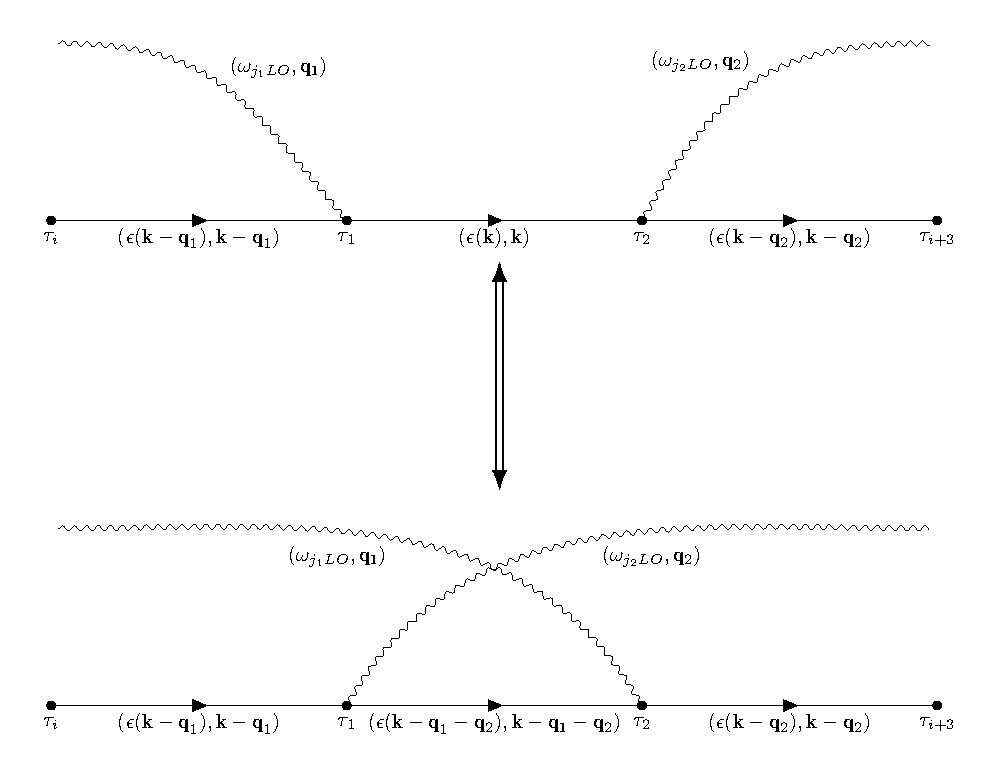
\includegraphics[scale=0.6]{swap_update.pdf}
    \caption{Diagram swap update.}
    \label{fig:swap_diagram}
\end{figure}
Let us call the two phonon propagator that we want to swap 1 and 2. We have that the two phonon propagators have momentum $\mathbf{q}_1$ and $\mathbf{q}_2$ with 
energy $\omega_{j_1LO}$ and $\omega_{j_2LO}$ and imaginary time $\tau_1$ and $\tau_2$, given that the electron propagator between the two vertices has momentum $\mathbf{k}_{el}$ we have that 
the acceptance ratio of the update is simply given by the ratio between the 2 diagrams:
\begin{equation}
\begin{split}
    &R_{swap}=\frac{D_n^{\xi_n'}(\mathbf{k},\tau,...)}{D_n^{\xi_n}(\mathbf{k},\tau,...)}=\\
    &=\exp\left\{-\left(\epsilon(\mathbf{k}_{el}+c_1\mathbf{q}_1-c_2\mathbf{q}_2)-\epsilon(\mathbf{k}_{el})-(c_1\omega_{j_1LO}-c_2\omega_{j_2LO})\right)(\tau_2-\tau_1)\right\},
\end{split}
\end{equation}
where $c_1$ and $c_2$ are integer variables that store the type of the vertex ($c_i=+1$ for an outgoing vertex, linked to a vertex with time $\tau'>\tau_i$, -1 for an incoming one with $\tau'<\tau_i$).\\
The next class I update is the \textbf{shift phonon} update: in this update a single phonon interaction vertex $\tau_i$ is shifted between 
the two adjacent phonon vertices $\tau_{left}$ and $\tau_{right}$. Given $\mathbf{k}_{i-1}$ and $\mathbf{k}_i$ the momenta of the two free electron propagators 
that are linked to the phonon vertex we have that the new imaginary time value $\tau_i'$ is found as
\begin{equation}
    \tau_i'=\tau_{left}-\frac{\log{(1-r(1-e^{-\Delta E(\tau_{right}-\tau_{left})}))}}{\Delta E},
\end{equation}
where the value of $\Delta E$ is retrieved with the following relation
\begin{equation}
    \Delta E =\epsilon(\mathbf{k}_{i})+\epsilon(\mathbf{k}_{i-1})-c_i\omega_{j_iLO},
\end{equation}
where $c_i$ is the phonon vertex type (+1 for outgoing vertices, -1 for incoming ones). The update is always accepted as long that the new proposed value 
is not too close to the two extrema $<10^{-9}$.\\
The last update that was implemented is the \textbf{stretch diagram} update (class I). In this update the whole diagram is stretched or compressed
like a spring: each electron propagator, together with the phonon propagators whose vertices are to the left and to the right of said propagator.\\
The imaginary time value of each vertex is shifted (from the first vertex with time value $\tau_1$ to the last $\tau_{2n+1}=\tau$ length of the diagram, while the first vertex at 0 is of course fixed) 
using the following formula:
\begin{equation}
    \tau'_i=\tau'_{i-1}-\frac{\log{(1-r)}}{\epsilon(\mathbf{k}_{i-1})-\mu+\sum_j\omega_{jLO}n_j},
\end{equation}
where $n_j$ is the number of phonon propagator with mode $j$ that are "active" at the index $j$ (they were created to the left of the 
$i$ vertex and and annihilated to the right of it). The update is rejected only if each new proposed value $\tau_i'$ is too close to the previously proposed 
vertex $\tau_{i-1}'$ or if $\tau_i'\ge\tau_{i+1}$ next vertex in the diagram.\\
The full simulation decides which of the 8 updates to choose based on a uniform random variable $r$ in $[0,1]$.
\subsection{Collected quantities and MC estimators}
After having implemented the features of the Diagrammatic Monte Carlo simulation, methods to collect results and analyze them are necessary. 
The simplest estimator that can be built is an \textbf{histogram method} to reconstruct the shape of the Green's function that we are simulating: 
A fixed number of bins $N_{bins}$ from 0 to $\tau_{max}$ is set at the beginning of the simulation such as every bin has width $\Delta\tau=\tau_{max}/N_{bins}$ and is centered at the value
$\tau_{j}=j\tau_{max}/N_{bins}+\Delta\tau/2$ with $j$ integer between 0 and $N_{bins}-1$.\\
After every iteration of the simulation, the diagram length $\tau_k$ is given as input to the histogram: if the value $\tau_k$ falls in the range  
$(\tau_{j}-\Delta\tau/2,\tau_j+\Delta\tau/2)$ the number of counts $n_j$ is updated by 1.\\
At the end of the simulations we will have $N_{bins}$ each with a different number 
of counts $n_j$. The shape of the Green's function can already be assessed in this form, but to obtain the right value at each bin a normalization factor 
is needed: the obvious normalization factor that is needed is the bin width $\Delta\tau$, but is not enough to get the actual Green's function. In fact, 
given that we have fixed a maximum imaginary time value $\tau_{max}$, the obtained Green's function is actually normalized over the $(0,\tau_{max})$ range: 
this is not how the Green's function is defined, since its domain is $(0,+\infty)$. For this reason we exploit the properties of the 0-order diagrams $D_0(\mathbf{k},\tau)$, which we know to 
have the simple exponential form 
\begin{equation}
    D_0(\mathbf{k},\tau)=e^{-(\epsilon(\mathbf{k})-\mu)\tau},
\end{equation}
since we know how to integrate this function we can use the integral value $I_0$ of the zero order diagrams to reconstruct the correct normalization factor-
the integral value $I_0$ is the following
 is computed:
\begin{equation}
    I_0=\int_{0}^{\tau_{max}}e^{-(\epsilon(\mathbf{k})-\mu)\tau}d\tau=\frac{1-e^{-(\epsilon(\mathbf{k})-\mu)\tau_{max}}}{\epsilon(\mathbf{k})-\mu},
\end{equation}
and the Green's function has the value
\begin{equation}
    P(\mathbf{k},\tau_j)=\frac{n_jI_0}{N_0\Delta\tau},
\end{equation}
with $N_0$ number of 0-order diagrams in the simulation.\\
Although that it is possible to estimate the \textbf{ground state energy} $E_P(0)$ of the polaron (also known as the \textbf{zero-point renormalization} or \textbf{ZPR}), by 
fitting an exponential function to the Green's function estimated as previously mentioned for large $\tau$ values \cite{fehske2007computational}, we can build an exact estimator 
that is able to compute a value for the ground state energy that has no discretization errors (due to the finite width of the bins in the histogram).\\
The estimator follows from these considerations \cite{mishchenko2000diagrammatic}: given a quantity $A$ specified by the diagrammatic expansion 
\begin{equation}
    A=\sum_{\nu}D_A(\nu),
\end{equation}
with $D_A(\nu)$ diagrams for which the quantity $A$ is computed, $\nu$ internal variables of the histogram with summation over discrete variables and 
integration over continuous ones, and a similar quantity $B=\sum_{\nu}D_B(\nu)$ defined similarly, it is possible to estimate the ratio of the 
two quantities as 
\begin{equation}
\begin{split}
    &\frac{B}{A}=\frac{\left(\sum_{MC_{A}\{\nu\}}Q_\nu\right)}{\sum_{MC{A}\{\nu\}}1}=\left\langle Q_\nu \right\rangle_{MC},\\
    &Q_\nu=\frac{D_B(\nu)}{D_A(\nu)},
\end{split}
\end{equation}
with $MC_{A}\{\nu\}$ set of internal parameters generated during the Monte Carlo simulation.\\
Given the definition, it might not be clear how this expression is useful in order to build an exact energy estimator. To start let us 
consider the fact that the two quantities $A$ and $B$ are usually the same Green's function (same expansion of the internal variables) taken with some variations 
in the external parameters. For the ground state energy this reduces to
\begin{equation}
    Q_\nu=\frac{P(\mathbf{k},(1+\lambda)\tau)}{P(\mathbf{k},\tau)}\to \exp{\left(-\lambda E_P(\mathbf{k})\tau\right)}
\end{equation}
for large $\tau$ values and $lambda$ small parameter. If we approximate the exponential with a Taylor expansion in $\lambda$ we get
\begin{equation}
    \exp{\left(-\lambda E_P(\mathbf{k})\tau\right)}=1-\lambda E_P(\mathbf{k})\tau+O(\lambda^2).
    \label{lambda_energy_estimator}
\end{equation}
The quantity $Q_\nu$ can be diagrammatically expanded as
\begin{equation}
    Q_\nu=\frac{D_A(\nu)}{D_B(\nu)}=\frac{D_{n_\nu}^{\xi_{n_\nu}}(\mathbf{k},(1+\lambda)\tau,\nu)}{D_{n_\nu}^{\xi_{n_\nu}}(\mathbf{k},\tau,\nu)},
\end{equation}
where the $\nu$ are the (same) internal variables up to a $\lambda$ scaling factor.\\
Expliciting the ratio we get
\begin{equation}
    Q_\nu=(1+\lambda)^n\left\{\prod_{l}\exp{\left(-\epsilon(\mathbf{k}_l)\Delta\tau_l\right)}\prod_{m}\exp{\left(-\omega_{jLO}\Delta\tau_m\right)}\right\},
    \label{decomposition_estimator_energy}
\end{equation}
where the index $l$ lists the free electron propagators while $m$ the free phonon ones.\\
If we now impose $\lambda\to 0$ we get
\begin{equation}
    Q_\nu \xrightarrow[\lambda\to 0]{}1+\lambda\left(n-\sum_l\epsilon(\mathbf{k}_l)\Delta\tau_l-\sum_m\omega_{jLO}\Delta\tau_m\right)+O(\lambda^2),
\end{equation}
which, when compared with \ref{lambda_energy_estimator}, gives the explicit expression for the energy estimator
\begin{equation}
    E_P(\mathbf{k})=\left\langle \frac{1}{\tau_k} \left(\sum_l\epsilon(\mathbf{k}_l)\Delta\tau_l-\sum_m\omega_{jLO}\Delta\tau_m-n_k\right) \right\rangle_{MC}\hspace{1cm}\tau_k\to+\infty
    \label{energy_estimator_MC}
\end{equation}
The ground state energy $E_P(0)$ is found for $\mathbf{k}=0$.\\
The next estimator that is defined is for the \textbf{effective mass} $m^*_p(\mathbf{k})$ of the polaron, which is in general anisotropic with respect to momentum (it 
has the same symmetry properties of the electron effective mass from which it is derived), its theoretical definition is
\begin{equation}
    \frac{1}{m^*_P(\hat{\mathbf{k}})}=\left(\frac{d^2 E_P(\mathbf{k})}{d{\mathbf{k}^2}}\right)_{\mathbf{k}=0}.
\end{equation}
While an effective mass exact estimator for the isotropic case has been derived \cite{mishchenko2000diagrammatic}, no attempts at defining it for the anisotropic 
case have been tried (at least to my knowledge). For this reason the following estimator has been developed: it should not be interpreted 
as a definite result and a more accurate expression is for sure obtainable.\\
We begin by noting that
\begin{equation}
\begin{split}
    Q_\nu=&\frac{P(\lambda\hat{\mathbf{e}},\tau)}{P(0,\tau)}\xrightarrow[]{\tau\to\infty}\hspace{5pt}\exp{\left\{-\left(E_P(\lambda\hat{\mathbf{e}})\tau-E_P(0)\right)\tau\right\}}=\\
    &=\exp{\left(-\frac{\lambda^2\tau}{2m^*_P(\hat{\mathbf{e}})}-E_P(0)\tau+E_P(0)\tau\right)}=\exp{\left(-\frac{\lambda^2\tau}{2m^*_P(\hat{\mathbf{e}})}\right)},
\end{split}
\end{equation}
which, for $\lambda\to 0$ becomes:
\begin{equation}
    \exp{\left(\frac{\lambda^2\tau}{2m^*_P(\hat{\mathbf{e}})}\right)}\xrightarrow[\lambda\to 0]{}1-\frac{\lambda^2\tau}{2m^*_P(\hat{\mathbf{e}})}+O(\lambda^4).
    \label{effective_mass_taylor}
\end{equation}
The ratio can be explicited in a similar way as it was done in \ref{decomposition_estimator_energy}:
\begin{equation}
    Q_\nu=\prod_l\exp\left\{-\frac{1}{2}\left[\frac{(\mathbf{k}_l+\lambda\hat{\mathbf{e}})^2}{m^*\left({\frac{\mathbf{k}_l+\lambda\mathbf{e}}{\sqrt{k^2_l+\lambda^2}}}\right)}-\frac{k^2_l}{m^*(\hat{k}_l)}\right]\Delta\tau_l\right\}.
    \label{decomposition_estimator_mass}
\end{equation}
The first electronic effective mass in this expression is problematic: the fact that $\lambda\to 0$ in the limit does not help with the evaluation since the mass only depends on the orientation of 
the momentum, for $\mathbf{k}\to 0$ (which is quite common) the expression is not defined without determining a clear $lambda$ value. For this reason 
we employ the approximation
\begin{equation}
    m^*\left({\frac{\mathbf{k}_l+\lambda\mathbf{e}}{\sqrt{k^2_l+\lambda^2}}}\right)\approx m(\hat{\mathbf{e}}).
    \label{effective_mass_approx}
\end{equation}
Using this expression \ref{decomposition_estimator_mass} becomes solvable at the price of losing accuracy. Given that conduction band minima usually have a prolate effective mass 
($m^*_x=m^*_y=m^*_{\perp}<m^*_z$) this means that our estimation sets an upper bound for the computed $m^*_z$ and a lower bound for $m^*_\perp$. In the case $m_x<m_y<m_z$ the behaviour 
of $m_y$ is not defined a priori.\\
Given \ref{effective_mass_approx}, \ref{decomposition_estimator_mass} becomes:
\begin{equation}
\begin{split}
    Q_\nu&=\prod_l\exp\left\{-\frac{1}{2m^*(\hat{\mathbf{e}})}\left[\mathbf{k}^2_l+\lambda(\mathbf{k}_l\cdot\hat{\mathbf{e}})+\lambda^2-k^2_l\right]\Delta\tau_l\right\}=\\
    &=\prod_l\exp\left\{-\frac{1}{2m^*(\hat{\mathbf{e}})}\left[\lambda(\mathbf{k}_l\cdot\hat{\mathbf{e}})+\lambda^2\right]\Delta\tau_l\right\},
\end{split}
\end{equation}
which for $\lambda\to 0$ becomes
\begin{equation}
    Q_\nu\xrightarrow[\lambda\to0]{}\hspace{5pt}1-\lambda\sum_l\frac{(\mathbf{k_l\cdot\hat{\mathbf{e}}})}{m^*(\hat{\mathbf{e}})}\Delta\tau_l - \lambda^2\sum_l\frac{\Delta\tau_l}{m^*(\hat{\mathbf{e}})}+\frac{\lambda^2}{2}\left(\sum_l\frac{(\mathbf{k_l\cdot\hat{\mathbf{e}}})}{m^*(\hat{\mathbf{e}})}\Delta\tau_l\right)^2+O(\lambda^3).
\end{equation}
Combining this equation with \ref{effective_mass_taylor} and identifying the corresponding $\lambda$ terms, we see that
\begin{equation}
    \frac{1}{m^*_P(\hat{\mathbf{e}})}=\frac{1}{m^*(\hat{\mathbf{e}})} - \frac{1}{m^*(\hat{\mathbf{e}})^2}\left \langle \frac{1}{\tau_k}\left(\sum_l(\mathbf{k}_l\cdot\hat{\mathbf{e}})\Delta\tau_l\right)^2   \right \rangle_{MC}.
\end{equation}
The formula for $m_{Px}^*$, $m_{Py}^*$ and $m_{Pz}^*$ are retrieved for $\hat{\mathbf{e}}=\hat{x}$, $\hat{\mathbf{e}}=\hat{y}$ and $\hat{\mathbf{e}}=\hat{z}$ respectively.\\
The last exact estimator which is shown is the Green's function exact estimator, which removes the discretization error in the Green's function 
estimation that is present in the histogram method, which inevitably introduces systematic errors.\\
We begin by observing that \cite{mishchenko2000diagrammatic}
\begin{equation}
    P(\mathbf{k},\tau_j)=\sum_\nu D(\mathbf{k},\tau_j,\nu)=\int d\tau \sum_\nu D(\mathbf{k},\tau,\nu)\delta(\tau-\tau_0),
\end{equation}
with $P(\tau_j)$ value of the Green's function at $\tau_j$.\\
Given a width $\Delta\tau$ fixed around the $\tau_j$ value (the procedure to define the $\tau_j$ values and the width $\Delta\tau$ is the 
same as previously done for the histogram method), we can define a Monte Carlo estimator for $P(\tau_j)$ as:
\begin{equation}
    P(\mathbf{k},\tau_j)=\left\langle  \frac{1}{\Delta\tau}\frac{D_{n_k}(\mathbf{k},\tau_k,...)}{D_{n_k}(\mathbf{k},\tau_j,...)} \theta\left(\left|\tau_k-\tau_j\right|-\frac{\Delta\tau}{2}\right)\right\rangle_{MC},
\end{equation}
where $\theta(\cdots)$ is the Heaviside step function, which takes into account only $\tau_k$ values that are inside the interval $(\tau_j-\frac{\Delta\tau}{2},\tau_j+\frac{\Delta\tau}{2})$.\\
In alternative, an estimator for $G^{(N)}(\mathbf{k},\tau_j)$ which only takes into account Diagrams with $N$ external phonons can be defined:
\begin{equation}
    G^{(N)}(\mathbf{k},\tau_j)=\left\langle  \frac{1}{\Delta\tau}\frac{D_{n_k}(\mathbf{k},\tau_k,...)}{D_{n_k}(\mathbf{k},\tau_j,...)} \theta\left(\left|\tau_k-\tau_j\right|-\frac{\Delta\tau}{2}\right)\delta_{N_k,N}\right\rangle_{MC},
\end{equation}
where the Kronecker delta $\delta_{N_k,N}$ only takes into account diagrams with $N_k=N$ number of external phonon propagators.